\documentclass[11pt, oneside]{article}   	% use "amsart" instead of "article" for AMSLaTeX format
\usepackage{geometry}                		% See geometry.pdf to learn the layout options. There are lots.
\geometry{letterpaper}                   		% ... or a4paper or a5paper or ... 
%\geometry{landscape}                		% Activate for for rotated page geometry
%\usepackage[parfill]{parskip}    		% Activate to begin paragraphs with an empty line rather than an indent
\usepackage{graphicx}				% Use pdf, png, jpg, or eps§ with pdflatex; use eps in DVI mode
								% TeX will automatically convert eps --> pdf in pdflatex		
\usepackage{amssymb}
\usepackage{amsmath}
\usepackage{setspace}
\usepackage[square,sort,comma,numbers]{natbib} \bibpunct{(}{)}{;}{author-year}{}{,} 
\usepackage[hidelinks]{hyperref}


\title{Local PCA Shows How Population Structure Differs Along the Genome}
\author{Han Li, Peter Ralph}
%\date{}							% Activate to display a given date or no date

\usepackage{color}
\newcommand{\plr}[1]{{\em \color{blue} #1}}

\newcommand{\pcone}{PC1}
\newcommand{\pctwo}{PC2}
\newcommand{\pc}[1]{PC#1}
\newcommand{\given}{\,\vert\,}
\newcommand{\st}{\,\colon\,}
\renewcommand{\and}{\,\&\,}
\newcommand{\E}{\mathbb{E}}
\renewcommand{\P}{\mathbb{P}}
\DeclareMathOperator{\sgn}{sgn}
\DeclareMathOperator{\var}{Var}
\DeclareMathOperator{\cov}{Cov}
\DeclareMathOperator{\tr}{tr}


\begin{document}
\maketitle
%\section{}
%\subsection{}
\doublespacing


\section*{Abstract}

Dimension reduction techniques,
such as principal component analysis (PCA),
are often used to discover and display large-scale structure in genomic datasets
found in the patterns of kinship
between the genotyped individuals,
and to control for the confounding effects of population structure in genome-wide association studies.
The genome-wide mean kinship that principal component uses
is an average of the relationships across all locus-specific genealogical trees.
However, many biological factors,
including linked selection,
can systematically skew patterns of kinship over intermediate genomic scales.
We show how to use principal components analysis (PCA) to describe this meso-scale variation in kinship,
and apply the method to genomic data from three species.
In each species we find that population structure varies on the scale of megabases to tens of megabases.
In a global human dataset, small, discontinuous variation is likely explained by polymorphic chromosomal inversions.
In a dataset of primarily African \textit{Drosophila melanogaster}, large, continuous variation across each chromosome arm
is explained by known chromosomal inversions thought to be under recent selection.
In a range-wide dataset of \textit{Medicago truncatula},
common axes of variation in population structure are shared between chromosomes,
correlate with local gene density,
and may be caused by background selection or local adaptation.
The method is a useful addition to the exploratory toolbox
of population genomics,
and is implemented as an R package.

\plr{Add percent of variance explained by first two MDS coordinates, after subtracting the genome-wide mean covariance matrix.}

\plr{Add references to supplemental whole-genome PCA plots in the text.}

\section{Introduction}

% The kinship matrix contains the kinship coefficient for pairwise individuals. 
% Kinship coefficient defines the genetic relatedness between individuals.
% It is the probability that two alleles randomly selected from two individuals are inherited from the most recent common ancester.
% It could be estimated from given pedigree or from genome-wide covariances of genotype markers. 
% It is well-known that for kinship matrix, actual relatednesses have a lot of noise about the expected value, and depend on where on the genome you look; this is why scans for selective sweeps work.
% Populations are often structured in some way while there are systematic genetic variation between populations. 


The phrase ``population structure'' refers to reduced gene flow between subpopulations, 
often because of geographical isolation.
However, it is widely recognized that because of selection the effects of gene flow are not equal everywhere on the genome,
and patterns of polymorphism and divergence can vary significantly depending on factors including local gene density.
This implies that, paradoxically, 
the population structure of a species depends on which part of the genome is being examined.

Population structure leads to systematic patterns in genome-wide mean kinship,
and so it is said that visualizations of kinship depict population structure,
rather than the \emph{effects} of population structure (which would be more accurate).
The \emph{kinship coefficient} for a pair of individuals
gives the expected proportion of their genome
that the two have inherited identically by descent;
for a single individual it is the inbreeding coefficient.
However, as \citet{wright1949genetical} wrote,
``It has probably occurred to the reader that the coefficient of inbreeding
may mean very different things in different cases.''
The kinship coefficient originally referred to the expected probability
of coinheritance within a given pedigree;
while modern applications to ``unrelated'' individuals
use a genetic covariance matrix to estimate the \emph{realized} proportion of the genome
coinherited from sufficiently recent ancestors.

Realized kinship summarizes the shapes
of the genealogical trees that relate the samples
at each location along the genome.
Since these trees vary along the genome, so does realized kinship;
but averaging over sufficiently many trees we hope to get a stable estimate,
independent of the genomic region chosen.
This hope is not entirely justified: for instance,
kinship on sex chromosomes is expected to differ from the autosomes;
and positive or negative selection on particular loci can dramatically disort shapes of nearby genealogies
\citep{maynardsmith1974hitchhiking,barton2000genetic,neher2013genetic,charlesworth2012effects},
and therefore patterns of kinship.
Indeed,
chromosome-scale variation in diversity and divergence has been observed in many species
\citep[e.g.][]{langley2012genomic};
species phylogenies can differ along the genome 
due to incomplete lineage sorting \citep[e.g.][]{pease2013accurate},
adaptive introgression and/or local adaptation \citep[e.g.][]{ellegren2012genomic,nadeau2012genomic,pool2015natural,vernot2014resurrecting};
and theoretical expectations predict that geographic patterns of relatedness should depend on selection
\citep{charlesworth2003review}.
Nonetheless, it is not generally known to what extent patterns of kinship vary along the genome,
nor what the major axes of variation are.


Patterns in genome-wide kinship are often summarized
by applying principal components analysis (PCA) \citep{patterson2006population} 
to the genetic covariance matrix,
as pioneered by \citet{menozzi1978synthetic}.
% About 37 years ago, \citet{menozzi1978synthetic} first applied principal component analysis (PCA) in population genetics to construct maps summarizing genetic variation \citep{menozzi1978synthetic}. 
% Nowadays, PCA is a widely used powerful non-parametric method to extract information from genetic data.  
% PCA results are derived from the covariance matrix of genotype matrix. 
The results of PCA can be directly related to the underlying genealogical history of the samples, 
such as time to most recent common ancestor and migration rate between populations \citep{novembre2008interpreting,mcvean2009genealogical}. 
These patterns are often geographical, producing ``maps'' of population structure
that reflect the samples' geographic origin distorted by rates of gene flow
\citep{novembre2008genes},
although other patterns emerge if recent migration or nongeographic kinship patterns are having a strong role in relatedness determining.
\citep{astle2009population}.
% Through dimension-reduction, PCA can identify key components of population structure, which describes how different samples are related, and are often closely related to geography. 
% Plots of the first two principal components (PCs) can mimic the samples' geographic origin to some extent. 
% Since population structure describes how different samples are related, samples living closer tend to be more genetically similar and thus tend to be clustered in PC plots \citep{novembre2008genes,patterson2006population}. 
% However this relatedness is limited while there's recent migration or for group with nongeographic kinship patterns,for example, social or religious groups. \citep{astle2009population}

As reviewed by \citet{astle2009population}, 
modeling ``background'' kinship between samples
is essential to successful genome-wide association studies,
and PCA has often been used for stratification correction \citep{price2006principal},
and so investigating variation in kinship along the genome can help us to have a
better understanding of the relation between genome structure 
and population structure, possibly leading to more powerful methods for association studies.

To investigate how population structure varies along the genome in several datasets, 
we cut each genome into windows (with hundreds to thousands of SNPs in each), 
applied PCA to each window, 
and visualized the major ways that population structure, as summarized by PCA, varies among windows.
% In this project, we used SNP data for human, \textit{Medicago truncatula}, and
whole genome sequencing data for \textit{Drosophila}.  
% Based on the principal components, we can estimate the similarity of population structure contained in each genome window.  
To quantify similarity of population structure between
windows, we constructed for each window an approximate, scaled covariance
matrix based on the first few principal components, and measured the pairwise Euclidean distance
between those matrices.  
We then use multidimensional scaling to visualize the
relationships between windows, which reduces the pairwise distance matrix to
lower dimension while preserving the distance information between windows as
well as possible \citep{borg2005modern}.  

% To interpret the results of MDS, we combine known genome feature information for each species, such as the
% distribution of inversions, and heterochromatin and gene density along the genome. 
Each species showed distinct patterns, reflecting differences in their biology;
before presenting results,
it may be helpful to have a prior idea of what factors are expected to affect population structure,
and how.
PCA summarizes patterns in kinship found in the genetic covariance matrix,
which is an average across locus-specific genealogies.
% However, different parts of genome have different genetic features. 
% First, each site of DNA may have different gene tree. 
% The covariance matrix of genotype matrix averages those gene trees. 
If individuals are closer in the genealogies of a given genomic region, 
they tend to be closer in the PCA maps for that region. 
% Different DNA segments may have different gene tree and therefore different population structure for those segments. 
% Second, the strength of linked selection differs for different DNA segments, and produces different population structure in region under linked selection compared to other region. 
% Selective sweeps cause local recent ancestry or short trees.
% Background selection causes shallow ones.
Strong selective sweeps of beneficial alleles can lead to relatively long genomic regions
characterized by short genealogical trees \citep{przeworski2005signature,garud2013selective}.
A genomic region with many targets for selection experiences
background selection and/or recurrent selective sweeps \citep{stephan1992effect,coop2012patterns},
which would tend to shorten genealogical trees in the region,
similar to a reduction in effective population size \citep{hudson1995deleterious,sattath2011pervasive}.
% Balancing selection causes deep trees.
On the other hand, balancing selection leads to very deep trees \citep{gao2014footprints},
and population structure locally describes which individuals have which alleles
rather than geographical proximity.
Finally, 
since recombination is suppressed between opposite orientations of a chromosomal inversion
near its breakpoints,
genealogies in these regions separate samples carrying the two orientations of the inversion.
In the resulting extended block, population structure shows two (for haploids) or three (for diploids) clusters
(indeed, \citep{ma2012investigation} has proposed using trimodality of local PCA plots
as a way to identify inversions).
% if a chromosomal inversion is polymorphic in the sample, 
% the regions around the breakpoints of inversions usually have high linkage disequilibrium and the two directions of a inversion will have different linked alleles around the breakpoints. Recombination suppression across inversions thus results in different genome structure and population structure. 
% Other effects, like noise, introgression might also influence population structure.
We will look for strong variation in population structure shared across large regions of the genome.
Many of the effects listed above (such as single selective sweeps or inversions) 
are not expected to have similar effects on population structure in different regions of the genome
because of randomness in which samples end up in which group;
but if these coincide with a region of reduced recombination (such as an inversion),
these could drive major patterns of variation.
The more subtle effects of genome-wide linked selection could be shared across large regions
due to large-scale variation in gene density
(as by background selection or local adaptation at many genes).


We chose PCA to summarize population structure,
but other methods, such as STRUCTURE \citep{falush2003inference},
SPA \citep{yang2012modelbased},
SpaceMix \citep{bradburd2015spatial},
or other matrix factorization methods \citep{engelhardt2010analysis}
would highlight different sources of variation in the data.
% There are other methods for visualizing population structure are like STRUCTURE,
% \citep{pritchard2000inference,falush2003inference, falush2007inference,hubisz2009inferring} 
% model-based approach,
% maps of heterozygosity
% \citep{ramachandran2005support}. 

Finally, a number of general methods for dimensionality reduction also use a strategy of ``local PCA''
\citep[e.g.][]{manjon2013diffusion,kambhatla1997dimension,weingessel2000local,roweis2000nonlinear},
performing PCA not on the entire dataset but instead on subsets of observations,
providing ``local'' pictures which are then stitched back together to give a global picture.
At first sight,
this differs from our use of the term in that we restrict to subsets of \emph{variables} instead of subsets of observations.
However, if we flip perspectives and think of each genetic variant as an observation,
our method shares common threads, although the ultimate goals and methods for visualization are different.
Future methods for visualization of genomic data
may benefit from other advances in this substantial literature 
\citep[reviewed in][]{vandermaaten2009dimensionality}.



\section{Methods}

The general steps in our method could be carried out in many ways.
Referring to Figure \ref{fig:diagram}, these are
(1) divide the genome into windows,
(2) summarize the patterns of relatedness (population structure) in each window,
(3) measure dissimilarity in population structure between each pair of windows,
(4) visualize the resulting dissimilarity matrix,
and (5) combine similar windows to more accurately estimate local population structure.
Details of how we carried these out are given below.

\begin{figure}
    \begin{center}
       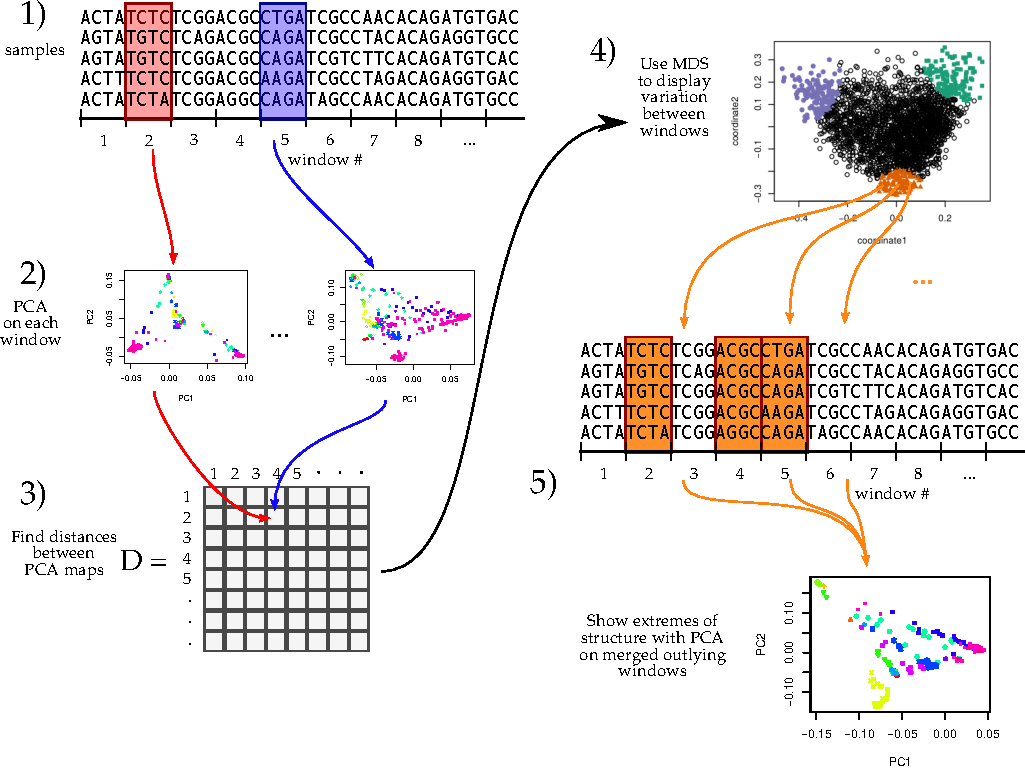
\includegraphics{the-method-diagram}
    \end{center}
    \caption{
         An illustration of the method; see text for details.
         % (1) the genome is divided into windows;
         % (2) population structure is summarized in each with PCA, and 
         % (3) dissimilarities for each are computed;
         % (4) the patterns of dissimilarity are visualized with MDS,
         % and (5) genomic regions clustering together are aggregated and visualized, again with PCA.
         \label{fig:diagram}
    }
\end{figure}



\subsection{Datasets}
% Recode the DNA sequence to a matrix consisting of 0,1,2 (and NA).

We used three publically available datasets (summarized in Table \ref{tab:data_stats});
as usual for genetic data we converted the data to a numeric matrix
(with one row per polymorphic variant and one column per sample)
by replacing each genotype with the number of nonreference alleles
(or NA for missing data).
A normalization step (see below) ensures the result does not depend on the choice of reference allele.

\paragraph{Human:}
We used genomic data from the entire POPRES dataset \citep{nelson2008population},
which has array-derived genotype information for 447,267 SNPs across the autosomes
of 3,965 samples in total: 346 African-Americas, 73 Asians, 3,187 Europeans and 359 Indian Asians.
(We excluded the sex chromosomes and the mitochondria.)
We use the allele that has highest frequency in the samples as the reference allele for each position. 

\paragraph{\textit{Drosophila melanogaster}:}
We also used whole-genome sequencing data from Drosophila Population Genomics Project (DPGP) \citep{lack2015drosophila}, 
which together has 380 samples from 16 countries across Africa and Europe.
\plr{Check: are all of our samples described in \citet{lack2015drosophila}? If yes, just say DPGP; if no, add appropriate citation (ask John what this should be). Also, add website?}
Since the \textit{Drosophila} samples are from inbred lines, we treat the samples as haploid when recoding;
regions with residual heterozygosity were marked as missing in the original dataset.
Each chromosome arm we investigated (Chr2L, Chr2R, Chr3L, and Chr3R) has 2--3 million SNPs.
Due to high density of missing data for some parts in the genome, 
we first deleted any samples with more than 8\% missing genotypes, 
and then deleted positions with more than 20\% missing data. 
(We chose these cutoffs as the tails of the relevant empirical distributions.)

\paragraph{\textit{Medicago truncatula}:}
Finally, we used whole-genome sequencing data from the \textit{Medicago truncatula} Hapmap Project \citep{tang2014improved},
which has 263 samples from 24 countries,
primarily distributed around the Mediterranean basin.
Each of the 8 chromosomes has 3-5 million SNPs;
we did not use the mitochondria or chloroplasts.

\begin{table}[ht]
\centering
    \begin{tabular}{p{0.8in}rrrr}
  \hline
    species 
    & \parbox[t]{.8in}{\# SNPs per \\ window} 
    & \parbox[t]{1in}{mean window\\ length (bp)}
    & \parbox[t]{1.2in}{mean \# windows \\ per chromosome} 
    & \parbox[t]{1.4in}{mean \% variance ex-\\plained by top 2 PCs} \\ 
  \hline
  Human & 100 & 636,494 & 203 & 0.55 \\ 
  \textit{Drosophila melanogaster} & 1,000 & 9,019 & 2,674 & 0.53 \\ 
  \textit{Medicago truncatula} & 10,000 & 102,580 & 467 & 0.50 \\ 
   \hline
\end{tabular}
\caption{
    Descriptive statistics for each dataset used,
    with the chosen window sizes.
    See text for how window sizes were chosen;
    in each window we performed PCA,
    computed the percent varince explained by the top two principal components;
    the mean across windows is given in the last column.
    \label{tab:data_stats}
}
\end{table}


\subsection{PCA in genomic windows}

After recoding, we divided the genome into contiguous segments (``windows''; see below),
% recoded matrix into contigous matrices that have the same columns but fewer rows than the original matrix, 
and applied Principal Component Analysis (PCA) as described in \citet{mcvean2009genealogical}
separately to the submatrices that corresponded to each window.
Specifically, we did PCA as follows:
denote by $Z$ the $L\times N$ recoded genotype matrix ($L$ is the number of SNPs and $N$ is the sample size), 
and by $\overline{Z_{s}}$ the mean of non-missing entries for allele $s$, 
so that $\overline{Z_{s}}=\frac{1}{n_s}\sum_j Z_{sj}$, 
where the sum is over the $n_s$ nonmissing genotypes.
We first compute the mean-centered matrix $X$, as $X_{si}=Z_{si}-\overline{Z_{s}}$,
and preserving missingness.
(This mean-centering makes the result not depend on the choice of reference allele,
exactly if there is no missing data, and approximately otherwise.)
Next, we find the covariance matrix of $X$, denoted $C$,
as $C_{ij} = \frac{1}{m_{ij}-1} \sum_s X_{si} X_{sj} - \frac{1}{m_{ij}(m_{ij}-1)} (\sum_s X_{si})(\sum_s X_{sj})$,
where all sums are over the $m_{ij}$ sites where both sample $i$ and sample $j$ have nonmissing genotypes.
\plr{Is that correct? This is not $X^T X/(m-1)$, which is what was here before, 
     but is what cov(), use='pairwise' does: see \url{package/tests/testthat/test_covariance.R}.}
% We compute the covariance matrix using the R function cov() , with use=``pairwise",
% which computes the covariance between each pair of individuals using all complete pairs of SNPs on those individuals.
The principal components are the eigenvectors of $C$, 
normalized to have Euclidean length equal to one,
and ordered by magnitude of the eigenvalues.

The top few principal components generally display population structure; 
we usually use the first two (referred to as $\pcone$ and $\pctwo$).
The above procedure can be performed on any subset of the data;
for future reference, denote by $\pcone_j$ and $\pctwo_j$
the result after applying to all SNPs in the $j^\text{th}$ window.

\plr{I'm talking about flipping signs up here, even though in the code we do it when computing variances. Do you think it makes sense here?}
Since eigenvectors are still only defined up to sign,
when comparing between windows we choose the sign to best match each other:
after choosing $\pcone_1$, for instance, and $u$ is the first eigenvector obtained from the covariance matrix
for window $j$,
then $\pcone_j = \pm u$,
where the sign is chosen according to which of 
$\sum_i (\pcone_{i1} - u_i)^{2}$ or
$\sum_i (\pcone_{i1} + u_i)^{2}$ 
is smaller.

\subsection{Choosing window length}

The choice of window length entails a balance between several factors.
In very short windows, genealogies of the samples will only be represented by a few trees,
so variation between windows represents demographic noise rather than meaningful variation in population structure.
Longer windows generally have more distinct trees (and SNPs), 
allowing for less noisy estimation of local population structure.
However, to better resolve meaningful signal, i.e., differences in population structure along the genome, 
we would like reasonably short windows.
Window length choice therefore entails a signal versus noise tradeoff
in the estimates of population structure.
% If we use the first principal component as a measure of population structure, 
% then to choose the best window length,
% we need to find a balance between the standard error of the first principal components for each window 
% and the standard deviation between windows. 
Since we summarize population structure using relative positions in the principal component maps,
we quantify ``noise'' as the standard error of a sample's position on PC1 in a particular window,
averaged across windows and samples,
and ``signal'' as the standard deviation of the sample's position on PC1 over all windows,
averaged over samples.
(Recall that the signs for PCs are chosen to match each other.)
Then, the mean variance across windows is
\begin{align*}
    \sigma_\text{signal}^2
    = 
    \frac{1}{N} \sum_{j=1}^{N}
        \frac{1}{L}\sum_{i=1}^{L}\left ( \pcone_{ij} -\overline\pcone_{j} \right )^{2} ,
\end{align*}
where $\overline\pcone_j = (1/N) \sum_{j=1}^N \pcone_{ij}$.
We estimate the standard error for each $\pcone_{ij}$ using the block jackknife \citep{efron1982jackknife}:
we divide the $j^\text{th}$ block into 10 equal-sized pieces,
and let $\pcone_{ij,k}$ denote the first principal component of this region found after removing the $k^\text{th}$ piece;
then the estimate of the squared standard error is
$\sigma^2_{ij} = \frac{9}{10} \sum_{k=1}^{10} ( \pcone_{ij,k} - \frac{1}{10} \sum_{\ell=1}^{10} \pcone_{ij,\ell} )^2$,
and we measure noise by averaging over samples and windows:
\begin{align*}
    \sigma^2_\text{noise}
    &=
    \frac{1}{N} \sum_{j=1}^{N} \frac{1}{L}\sum_{i=1}^{L} \sigma^2_{ij} .
\end{align*}

We calculated $\sigma^2_\text{signal}$ and $\sigma^2_\text{noise}$
for a range of window sizes,
and for our main results
chose the smallest window for which $\sigma^2_\text{signal}$ was consistently larger than $\sigma^2_\text{noise}$;
the values for various window sizes across \textit{Drosophila} chromosomes are shown in Table \ref{tab:window_sizes},
and the choices for all taxa are in Table \ref{tab:data_stats}.
In practice, even substantially different window sizes result in the same genome-wide patterns.
We also chose windows to each consist of the same number of neighboring SNPs.
We compared to the results when windows are each of the same physical length (in bp) but of the same average length,
and results were nearly identical.

% # Variances within and between windows for Drosophila, multiplied by 1000:
% w <- structure(list(chrom = structure(c(1L, 1L, 2L, 2L, 3L, 3L, 4L, 
% 4L, 5L, 5L), .Label = c("2L", "2R", "3L", "3R", "X"), class = "factor"), 
%     type = structure(c(1L, 2L, 1L, 2L, 1L, 2L, 1L, 2L, 1L, 2L
%     ), .Label = c("noise", "signal"), class = "factor"), `100` = c(2.05209, 
%     2.75625, 2.18089, 2.77729, 2.07936, 2.601, 1.95364, 2.58064, 
%     2.48004, 2.61121), `500` = c(1.64025, 2.69361, 1.91844, 2.704, 
%     1.99809, 2.52004, 1.764, 2.51001, 2.04304, 2.43049), `1000` = c(1.18336, 
%     2.22784, 1.63216, 2.65225, 1.64025, 2.401, 1.43641, 2.44036, 
%     1.53664, 2.304), `10000` = c(0.169, 0.676, 0.576, 2.31361, 
%     0.73441, 1.681, 0.58564, 1.96249, 1.61604, 0.324), `1e+05` = c(0.03969, 
%     0.31329, 0.13456, 1.82329, 0.24649, 1.89225, 0.20164, 1.39876, 
%     0.169, 1.14244)), .Names = c("chrom", "type", "100", "500", 
% "1000", "10000", "1e+05"), row.names = c(NA, -10L), class = "data.frame")
% print(xtable(w),include.rownames=FALSE)

\begin{table}[ht]
\centering
    \begin{tabular}{cccrrrrr}
  \hline
        & & & \multicolumn{5}{c}{window length (SNPs)} \\
 & chrom.\ arm  & & 100 & 500 & 1,000 & 10,000 & 100,000 \\ 
  \hline
    & 2L & $\sigma^2_\text{noise}$  & 2.05  &  1.64  &  1.18  &  0.17  &  0.04 \\
    & 	 & $\sigma^2_\text{signal}$ & 2.76  &  2.69  &  2.23  &  0.68  &  0.31 \\
    & 2R & $\sigma^2_\text{noise}$  & 2.18  &  1.92  &  1.63  &  0.58  &  0.13 \\
    & 	 & $\sigma^2_\text{signal}$ & 2.78  &  2.70  &  2.65  &  2.31  &  1.82 \\
    & 3L & $\sigma^2_\text{noise}$  & 2.08  &  2.00  &  1.64  &  0.73  &  0.25 \\
    & 	 & $\sigma^2_\text{signal}$ & 2.60  &  2.52  &  2.40  &  1.68  &  1.89 \\
    & 3R & $\sigma^2_\text{noise}$  & 1.95  &  1.76  &  1.44  &  0.59  &  0.20 \\
    & 	 & $\sigma^2_\text{signal}$ & 2.58  &  2.51  &  2.44  &  1.96  &  1.40 \\
    & X  & $\sigma^2_\text{noise}$  & 2.48  &  2.04  &  1.54  &  1.62  &  0.17 \\
    & 	 & $\sigma^2_\text{signal}$ & 2.61  &  2.43  &  2.30  &  0.32  &  1.14 \\
   \hline
\end{tabular}
\caption{
    Measures of signal and noise,
    computed separately for each chromosome arm in the \textit{Drosophila} dataset,
    at different window sizes.
    All values are multiplied by $1,000$
    (so typical variation is of order of 50\% of the actual values).
    Starting at windows of 1,000 SNPs, the signal (variation of PC1 between windows)
    starts to be substantially larger than the noise (standard error of PC1 for each window).
} \label{tab:window_sizes}
\end{table}



\subsection{Similarity of population structure between windows}

We think of local population structure as being summarized by \emph{relative} position of the sampmles
in the space defined by the top principal components.
Since rotations of this space imply identical population structure,
we do not compare population structure of different genomic windows using the PCs directly, 
but instead compare the low-dimensional approximations of the local covariance matrices
obtained using the top $k$ PCs.
(For results shown here, we use $k=2$;
results using larger numbers of PCs were nearly identical.)
We do this, rather than using the entire covariance matrix, 
both for computational efficiency 
and because the top PCs summarize important population structure, 
so using only these should reduce the effect of noise.
To remove the effect of variation in mutation rate between windows,
we also rescale each covariance matrix so that the underlying data matrix has trace norm equal to one.
To do this, define the $N \times k$ matrix $V(i)$ so that the $\ell^\text{th}$ column of $V(i)$
is equal to the $\ell^\text{th}$ princpal component of the $i^\text{th}$ window,
multiplied by $\sqrt{ \lambda_{\ell i} / \sum_{m=1}^k \lambda_{m i} }$.
% \begin{equation}
%     \begin{aligned}
%         V_{i1}&=\sqrt{\frac{\lambda _{1i}}{\lambda _{1i}+\lambda _{2i}}}PC1_{i} ,
%         \qquad
%         V_{i2}&=\sqrt{\frac{\lambda _{2i}}{\lambda _{1i}+\lambda _{2i}}}PC2_{i} 
%     \end{aligned}
% \end{equation}
Then, the rescaled, $k$-dimensional covariance matrix for the $i^\text{th}$ window is
\begin{align}
    M(i) &= \sum_{\ell=1}^k V_{i\ell} V_{i\ell}^T .
\end{align}
% \begin{align}
%     M_{i} &= \frac{\lambda_{1i}PC1_{i}PC1_{i}^{T}+\lambda_{2i}PC2_{i}PC2_{i}^{T}}{\lambda_{1i}+\lambda_{2i}} 
% \end{align}

We then use
Euclidean distance $D_{ij}$ between the matrices $M(i)$ and $M(j)$ 
to measure the similarity of population structure for the $i^\text{th}$ window and $j^\text{th}$ window. 
Since 
$\sum_{ij} (A_{ij}-B_{ij})^2 = \sum_{ij} (A^2_{ij} + B^2_{ij}) - 2 \tr(A^T B)$,
and $M(i) = V(i) V(i)^T$,
then due to the orthogonality of eigenvectors and the cyclic invariance of trace,
$D_{ij}$ can be computed efficiently as
\begin{align}
    D_{ij} 
    = 
    \frac{ \sum_{\ell=1}^k \lambda_{\ell i}^2 }{ (\sum_{\ell=1}^k \lambda_{\ell i})^2 }
    + \frac{ \sum_{\ell=1}^k \lambda_{\ell j}^2 }{ (\sum_{\ell=1}^k \lambda_{\ell j})^2 }
    - 2 \sum_{\ell, m=1}^k (V(i)^T V(j))^2_{\ell m} .
\end{align}
% from the code for pc_dist():
% #' In the unweighted case, suppose that (u) and (v) are sets of vectors, and that 
% #'    A = a_1 * u_1 u_1^T + ... + a_j * u_j u_j^T = U diag(a) U^T
% #'    B = b_1 * v_1 v_1^T + ... + b_j * v_k v_k^T = V diag(b) V^T,
% #' where U is the matrix whose columns are (u), and likewise for V.
% #' Then 
% #'    (A-B)^T (A-B) = A^T A + B^T B - A^T B - B^T A
% #' and so
% #'    ||A-B||^2 = ||A||^2 + ||B||^2 - 2 tr( A^T B )
% #' By the cyclic invariance of trace, if X = U^T V then
% #'    tr( A^T B ) = tr( U diag(a) U^T V diag(b) V^T ) = tr( diag(a) X diag(b) X^T ) .
% \begin{align}
%     \begin{split}
%     D_{ij} &= 
%         \left \{
%                 \left ( 
%                     V_{i1}\cdot V_{i1}^{} 
%                 \right )^{2}
%                 + \left ( V_{i2}\cdot V_{i2}^{} \right )^{2}
%                 + \left ( V_{j1}\cdot V_{j1}^{} \right )^{2} 
%                 +\left ( V_{j2}\cdot V_{j2}^{} \right )^{2} 
%         \right. \\ 
%         & \left. \qquad {}  
%             -2\left [ 
%                 \left ( V_{i1}\cdot V_{j1}^{} \right )^{2}
%                 + \left ( V_{i1}\cdot V_{j2}^{} \right )^{2}
%                 + \left ( V_{i2}\cdot V_{j1}^{} \right )^{2} 
%                 + \left ( V_{i2}\cdot V_{j2}^{} \right )^{2}
%             \right ]
%         \right \}^{1/2}
%     \end{split}
% \end{align}


\subsection{Visualization of results}

We use multidimensional scaling (MDS) to visualize relationships between windows
as summarized by the dissimilarity matrix $D$,
that produces a set of $m$ coordinates for each window that
give the arrangement in $m$-dimensional space that best recapitulates the original distance matrix.
For results here, we use $m=2$ to produce one- or two-dimensional visualizations of relationships between windows' population structure.

We then locate variation in population structure along the genome
by choosing collections of windows that are nearby in MDS cooridinates,
and map their positions along the genome.
Their common population structure is identified by extracting the corresponding genomic regions
and performing PCA on all, aggregated regions.


\subsection{Software}

The methods described here
are implemented in an open-source R package
available at \url{https://github.com/petrelharp/lostruct},
as well as scripts to perform all analyses from VCF files
at various parameter settings.


%%%%%%%%%%%%%%%%%%%%%%%%%%%%%%
\section{Results}

In these three species, PCA plots vary along the genome in a systematic way, showing strong chromosome-scale correlations.
This implies that variation is due to meaningful variation in population structure, 
since fluctuations due to demographic noise are not expected to show long distance correlations. 
Below, we discuss the results and likely underlying causes.


%%%%%%%%%%%
\subsection{\textit{Drosophila melanogaster}}

We ran the method on chromosome arms 2L, 2R, 3L, 3R and X separately. 
For each, the two-dimensional MDS visualization resembles a triangle,
as seen in Figure \ref{fig:mds_chr2L}.
Since the relative position of each window in this plot shows the similarity between windows, 
this suggests that there are at least three extreme types of population structure 
typified by windows found in the three corners of the triangle,
and that other windows' population structure may be a mixture of those extremes. 

\begin{figure}
    \begin{center}
       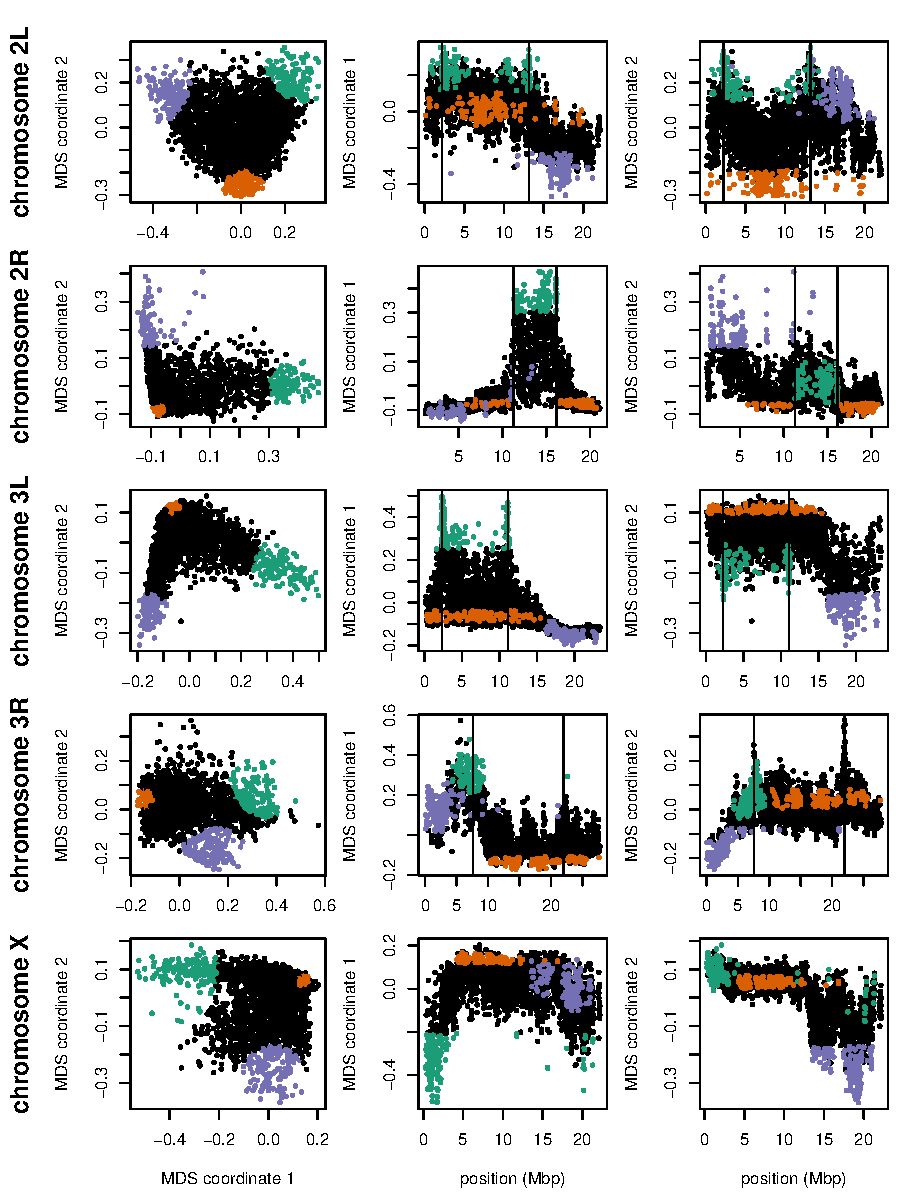
\includegraphics{Fig1_allchr_Together_MDS_plot_compact}
    \end{center}
    \caption{
        Variation in structure for windows across \textit{Drosophila melanogaster} chromosome arms.
        In all plots, each point represents one window along the genome.
         The first column shows the MDS visualization of relationships between windows,
         and the second and third columns show the position (midpoint) of each window along the genome
         against the first and second MDS coordinates, respectively. 
         Rows show results from different chromosome arms, from top to bottom these are 2L, 2R, 3L, 3R, and X. 
         Colors are consistent for plots in each row. 
         Vertical black lines show the breakpoints of known polymorphic inversions
         (from top to bottom: In(2L)t, In(2R)NS, In(3L)OK, In(3R)K).
         \label{fig:mds_chr2L}
    }
\end{figure}


To investigate these extremes, for each chromosome arm we visually selected three ``extreme'' windows in the MDS plot,
and take out the 5\% of windows that are closest to it in the MDS coordinates;
highlighted these windows' positions along the genome (colors in Figure \ref{fig:mds_chr2L}),
and produced PCA plots for each collection of windows
(shown in Figure \ref{fig:pca_by_pop}).


\begin{figure}
    \begin{center}
       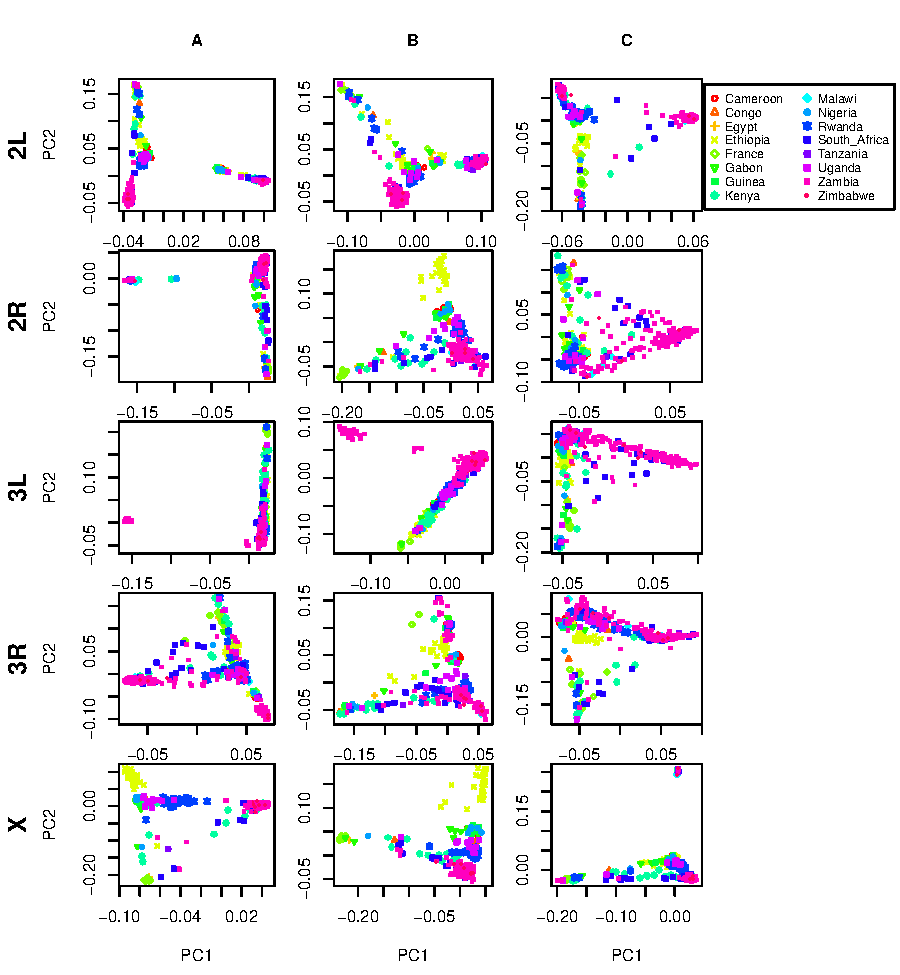
\includegraphics[width=1\textwidth]{Fig2_pca_plots_allchr_3peaks_label_update}
    \end{center}
    \caption{      
        PCA plots for the three sets of genomic windows colored in Figure \ref{fig:mds_chr2L},
        on each chromosome arm of \textit{Drosophila melanogaster}.
        In all plots, each point represents a sample. 
        The first column shows the combined PCA plot for windows 
        whose points are colored green in Figure \ref{fig:mds_chr2L}; 
        the second is for orange windows; 
        and third is for purple windows.
         \label{fig:pca_by_pop}
    }
\end{figure}


The variation in population structure turns out to be almost entirely explained by
several large inversions that are polymorphic in these samples, identified in \citet{corbett2012population}. 
Frequencies of each inversion in the sample are given in Table \ref{tab:inversion_freqs}.
\plr{Add this table.}
We recolored the PCA plots in Figure \ref{fig:pca_by_pop} by the orientation of the inversion for each sample,
obtaining Figure \ref{fig:pca_by_inversion}.
Taking chromosome arm 2L as an example,
the two regions of similar, extreme population structure
shown in green in the first row of Figure \ref{fig:mds_chr2L}
lie directly around the breakpoints of the iversion In(2L)t,
and the PCA plots in the first rows of figure \ref{fig:pca_by_inversion}
shows that population structure here is mostly determined by inversion orientation.
The regions shown in purple lie near the centromere,
and have population structure reflective of two axes of variation,
seen in figure \ref{fig:pca_by_pop},
which correspond roughly to latitude within Africa and to degree of cosmopolitan admixture respectively
(see \citet{pool2015natural} for more details).
\plr{check that reference}
The regions shown in orange mostly lie inside the inversion,
and show population structure that is a mixture between the other two,
as expected due to recombination within the (long) inversion \citep{kirkpatrick2015chromosome}.
\plr{check that reference too}
Similar results are found in other chromosome arms,
\plr{add chromosome X}
except that the situation of Chr3R is a little more complicated,
due to the coexistence of two polymorphic inversions (In(3R)K and In(3R)P) at intermediate frequency.
However, peaks in MDS coordinates along the chromosome show the breakpoints of both,
although we have not highlighted portions of the MDS plot that pick these out.
Two further inversions, In(3L)P and In(3R)Mo, are at very low frequency in these samples, 
and do not significantly influence population structure.

\begin{figure}
    \begin{center}
       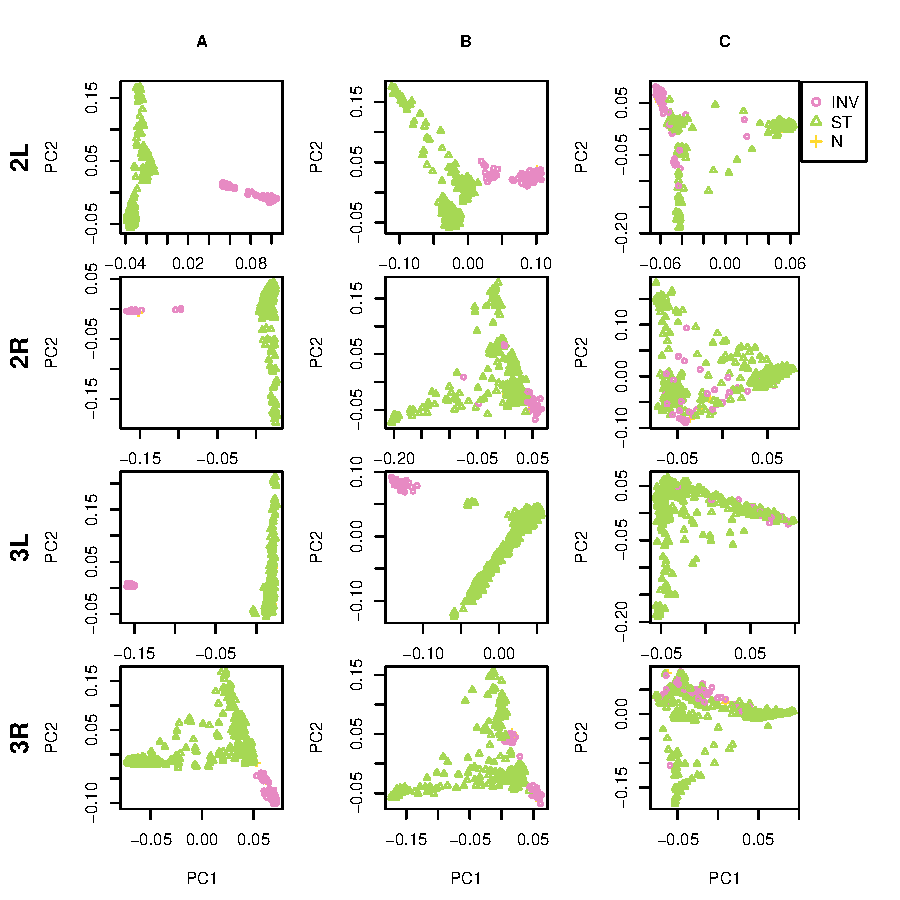
\includegraphics{Fig3_pca_plots_color_by_inv_allchr}
    \end{center}
    \caption{
         As in Figure 2, except that samples are colored by orientation of the corresponding polymorphic inversions, 
         In(2L)t, In(2R)NS, In(3L)OK and In(3R)K respectively. 
         (Data from \citet{lack2015drosophila}.
        \label{fig:color_inver}
    }
\end{figure}

%%%%%%%%%%%
\subsection{Human}

As for the \textit{Drosophila} data, we ran our method separately on all 22 human autosomes, 
with results shown in Supplementary Figure XXX.
\plr{Add plots for remaining autosomes to supplement.}
On each, variation in population structure was dominated by a small number of windows
having similar population structure to each other that differed dramatically from the rest of the chromosome.
Such regions seem to often coincide with inversions:
for instance, the eleven windows that are outliers in the first MDS coordinate of chromosome 8 (Figure \ref{fig:mds_human}b) 
coincide with the position of known polymorphic inversions on 8p23. 
Similar results are found in other chromosomes that have known inversions,
shown in Figure \ref{fig:mds_human}.
PCA plots of these windows show a characteristic trimodal shape,
presumably distinguishing samples having each of the three diploid genotypes for each inversion orientation
(although we do not have data on orientation status).
PCA has been previously proposed as a method to computationally identify inversions \citep{ma2012investigation},
but understanding how well the method can distinguish inversions from regions of low recombination
is beyond the scope of this paper.

We also ran the method on all 22 autosomes together, 
and found that, remarkably, 
the inversion on chromosome 8 is still the most striking outlying signal.
Further investigation with a denser set of SNPs,
allowing a finer genomic resolution,
may yield other patterns.

\begin{figure}
    \begin{center}
       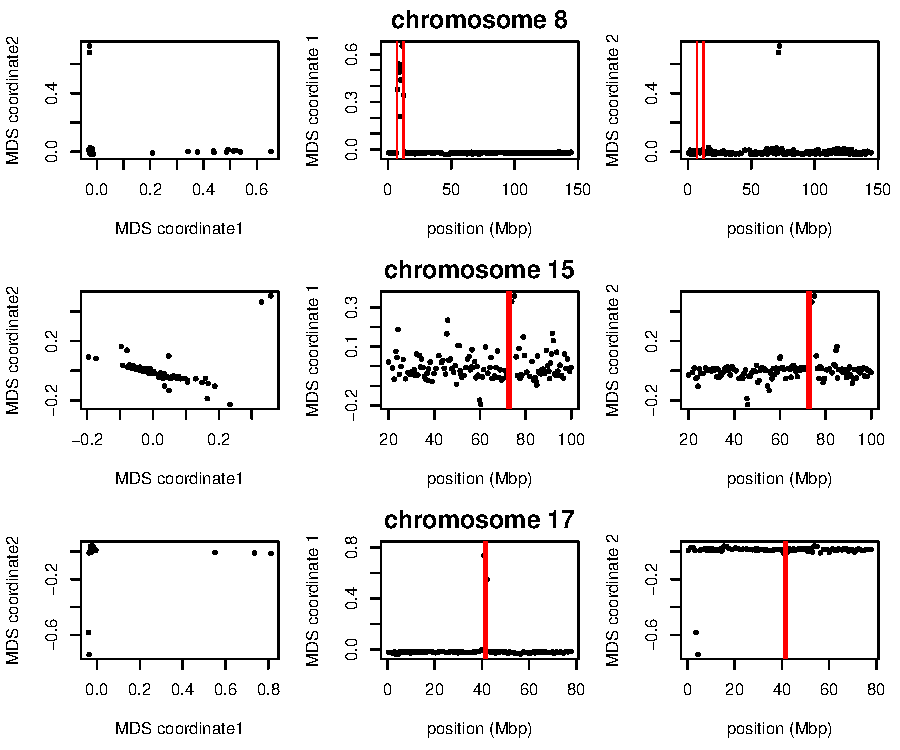
\includegraphics[width=0.9\textwidth]{Fig4_POPRES_Together_MDS_plot_chr8_15_17}
    \end{center}
    \caption{
         Variation in structure between windows on human chromosomes 8, 15, and 17. 
         Each point in each plot represents a window.
         The first column shows the MDS visualization of relationships between windows;
         the second and third columns show the two MDS coordinates of each window against its position (midpoint) along the chromosome. 
         Rows, from top to bottom show chromosomes 8, 15, and 17. 
         The vertical red lines show the breakpoints of known inversions from \citep{antonacci2009characterization},
         whose values are listed in \plr{add these in a table}.
        \label{fig:mds_human}
    }
\end{figure}


%%%%%%%%%%%
\subsection{\textit{Medicago truncatula}}

Unlike the other two species,
the method applied separately on all eight chromosomes of \textit{Medicago truncatula} 
showed similar patterns of gradual change in population structure across each chromosome,
with no indications of chromosome-specific patterns.
This consistency suggests that the factor driving the population structure for each chromosome is the same,
as might be caused by varying strengths of linked selection.
To verify that variation in population structure is shared across chromosomes,
we applied the method to all chromosomes together.
Results for chromosome 3 are shown in Figures \ref{fig:mds12_medicago} and \ref{fig:pca_medicago}
(other chromosomes are similar).

Across chromosomes, the high values of MDS coordinate 1 coincide with the position of the heterochromatic regions surrounding the centromere,
which often have lower gene density and may therefore be less subject to linked selection \citep{kulikova2001integration,paape2013selection}. 
To verify that this is a possible explanation,
we computed gene density near each window using gene models in Mt4.0 JBrowse \citep{tang2014improved}. 
\plr{Say exactly what was computed.}
These values are shown juxtaposed with
the first MDS coordinate of each window is shown in Figure \ref{fig:mds_medicago},
and are significantly correlated, as shown in Figure \ref{fig:mds_gene_count}.
Other genomic features covary with gene density, however,
so we cannot rule out alternative hypotheses.

We also found nearly identical results when choosing shorter windows of 1,000 SNPs;
or choosing windows of equal length in base pairs rather than SNPs.

\begin{figure}
    \begin{center}
       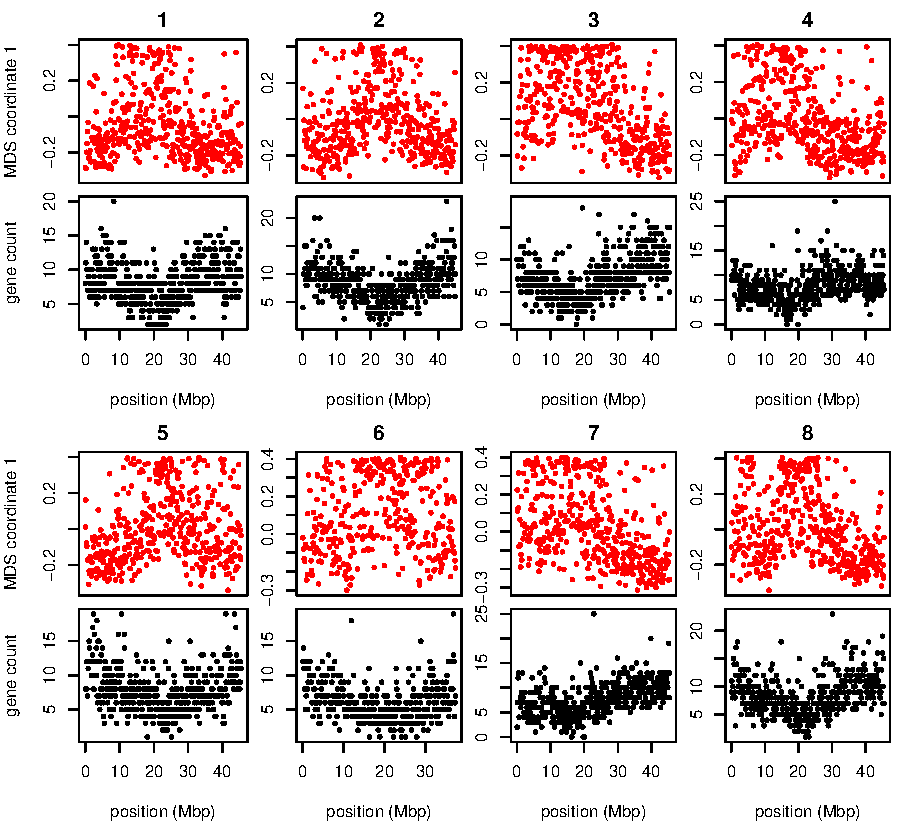
\includegraphics[width=0.9\textwidth]{Fig5_MDS_and_gene_count_allchr}
    \end{center}
    \caption{
         MDS visualization and gene density for each window in the \textit{Medicago} genome,
         for chromosomes 1--8 (numbered above each pair of figures).
         For each chromosome, the red plot above is first coordinate of MDS against the middle position of each window along each chromosome. 
         The black plot below is gene count for each window against the position of each window.
         \label{fig:mds_medicago}
    }
\end{figure}

\begin{figure}
    \begin{center}
       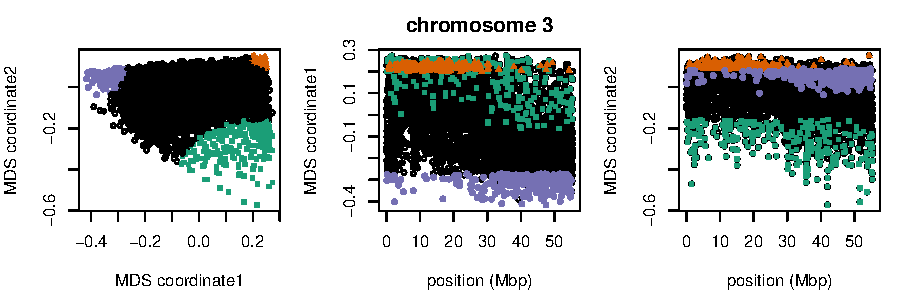
\includegraphics[width=0.9\textwidth]{Fig6_Together_MDS_plot_chr3_final}
    \end{center}
    \caption{
     MDS visualization for Medicago chromosome 3. Each point in the plot represents a window.
       \label{fig:mds12_medicago}
    }
\end{figure}

\begin{figure}
    \begin{center}
       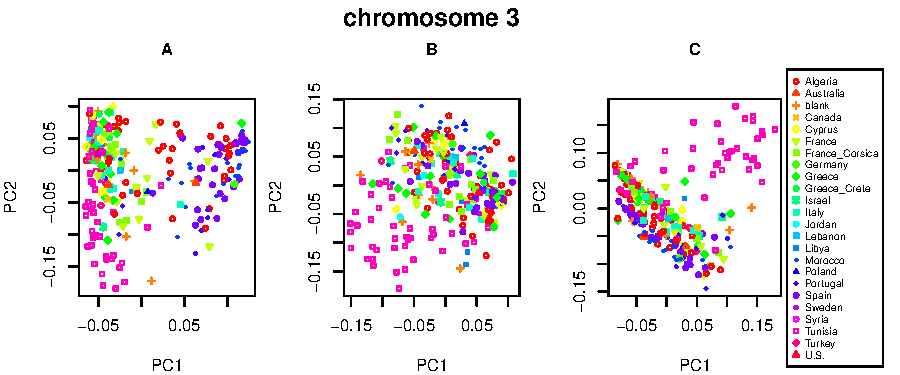
\includegraphics[width=0.9\textwidth]{Fig7_pca_plots_for_Medicago_chr3_3peaks_byMDS}
    \end{center}
    \caption{
        PCA plots for the sets of genomic windows colored (A) green, (B) orange, and (C) purple in Figure \ref{fig:mds12_medicago}. 
        Each point corresponds to a sample, colored by country of origin.
        \label{fig:pca_medicago}
    }
\end{figure}


\begin{figure}
    \begin{center}
       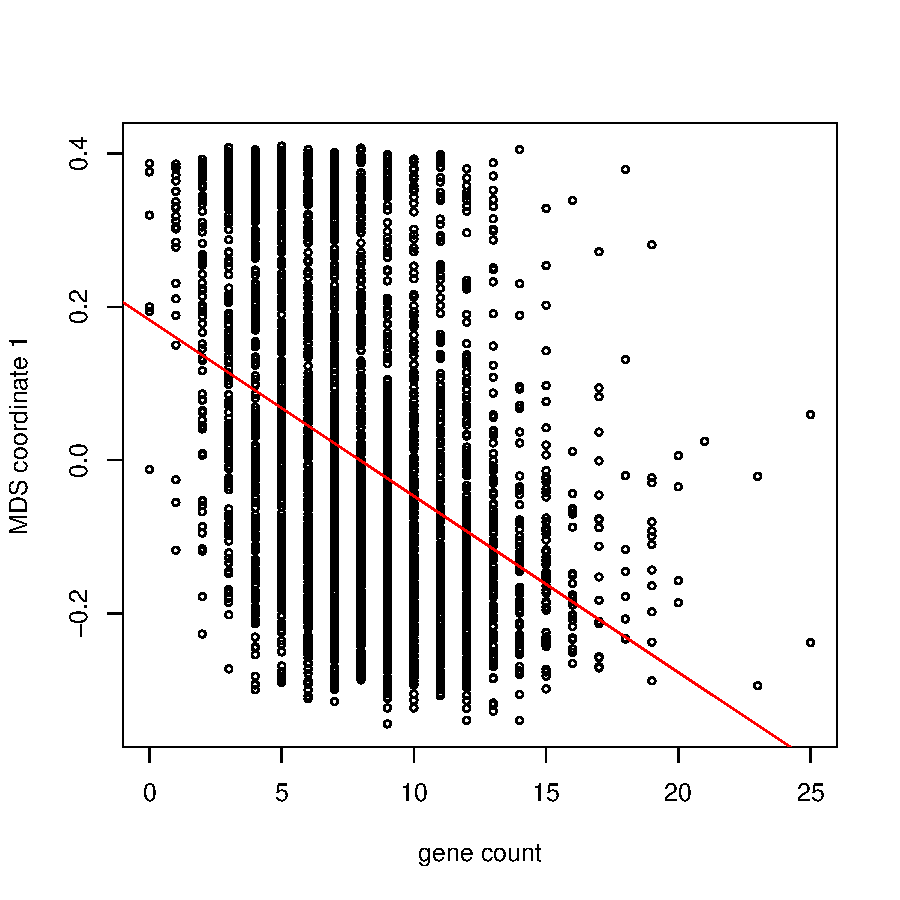
\includegraphics{MDS_1D_against_gene_count_all_chr_win104_with_lm}
    \end{center}
    \caption{
        First MDS coordinate against gene density for all 8 chromosomes. 
        The first MDS coordinate is significantly correlated with gene count ($r=0.146$, $p=2.2\times 10^{-16}$). 
        (See supplementary for each single chromosome's MDS result against gene count for \textit{Medicago})
        \label{fig:mds_gene_count}
    }
\end{figure}

%%%%%%% %%%%%%%%%
\section{Discussion}

Our investigations have found a remarkable amount of variation in population structure across the genomes
of three diverse species,
revealing distinct biological processes driving this variation in each species.
More investigation, particularly on more species and datasets will help uncover which patterns are generalizable.

With growing appreciation of the heterogeneous effects of selection across the genome,
especially the importance of adaptive introgression, hybrid speciation \citep{pool2015natural,brandvain2014speciation,hufford2013genomic,fitzpatrick2010rapid,staubach2012genome},
local adaptation \citep{lenormand2002limits,wang2014isolation},
and inversion polymorphisms \citep{kirkpatrick2015chromosome,kirkpatrick2010chromosome},
local PCA may prove to be a useful exploratory tool to discover important genomic features.
It is unclear whether the technique will be useful on reduced representation genotyping datasets 
due to marker density and issues with missing data --
our investigations with one such dataset were inconclusive --
but even low coverage, whole-genome sequence is very promising.


\paragraph{Confounding in GWAS}
So-called cryptic relatedness between samples
has been one of the major sources of confounding in genome-wide association studies (GWAS)
and so methods must account for it by modeling population structure or kinship \citep{gwas_confounding_review,mixed_models}.
Since population structure is not constant along the genome,
this could in principle lead to an inflation of false positives parts of the genome
with stronger population structure than the genome-wide average.
Fortunately, in our human dataset this does not seem likely to have a strong effect:
most variation is due to small, independent regions, possibly primarily inversions,
and so may not have a major effect on GWAS.
In the other species we examined, particularly \textit{Drosophila melanogaster},
treating population structure as a single quantity could be severely misleading.


\paragraph{Parameter choices}
There are several choices in the method that may affect the results.
As with whole-genome PCA,
the choice of samples is important,
as variation not strongly represented in the sample will not be discovered.
The effects of strongly imbalanced sampling schemes are often corrected by dropping samples in overrepresented groups;
but downweighting may be a better option that does not discard data.
Next, the choice of window size may be important,
although in our applications results were not sensitive to this,
indicating that the limit of resolution was smaller than the scale on which patterns of kinship varies along the genome.
Finally, which collections of genomic regions are compared to each other (steps 3 and 4 in figure \ref{fig:diagram}),
along with the method used to discover common structure,
will affect results.
We used MDS, applied to either each chromosome separately or to the entire genome;
for instance, human inversions are clearly visible as outliers when compared to the rest of their chromosome,
but genome-wide, their signal is obscured by the numerous other signals of comparable strength.

Besides window length, there is also the question of how to choose windows.
In these applications we have used nonoverlapping windows with equal numbers of polymorphic sites.
Alternatively, windows could be chosen to have equal length in genetic distance,
so that each would have roughly the same amount of phylogenetic information.
However, given the insensitivity of our results to window length,
this seems unlikely to give different results.

More generally, there are many possible methods to discover common structure in different parts of the genome.
The methods we chose discovered strong biological signal of different types in three datasets;
but it is possible that other methods for measuring dissimilarity between windows' covariance matrices
or for summarizing the matrix of pairwise distances between windows
would lead to different insights.
Minor points we have not explored include how to decide how many PCs to use in approximating structure of each window
(equations XX),
how many MDS coordinates to use when describing the distance matrix between windows,
or how to choose interesting regions of the genome when the MDS plot is not triangular.
These are all part of more general techniques in dimension reduction and high-dimensional data visualization;
we encourage the user to experiment.


\paragraph{Chromosomal inversions}
A major driver of variation in population structure in two datasets we examined are inversions.
This may be common,
but the example of \textit{Medicago truncatula} shows that polymorphic inversions are not ubiquitous.
PCA has been proposed as a method for discovering inversions \citep{ma2012investigation};
However, the signal left by inversions likely cannot be distinguished from long haplotypes under balancing selection 
or simply regions of reduced recombination.
However, in many applications, inversions are a nuisance.
For instance, SMARTPCA \citep{patterson2006population} reduces their effect on PCA plots
by regressing out the effect of linked SNPs on each other.
It would be interesting to see if smoehow removing the effects of inversions in the \textit{Drosophila melanogaster} or human datasets
would produce a pattern similar to that seen in \textit{Medicago truncatula}.

%%%%%%%%
\subsection*{Acknowledgements}

We are indebted to John Pool, Russ Corbett-Detig, Matilde Cordeiro, and Peter Chang 
for assistence with obtaining data and interpreting results
(especially inversion status of \textit{D.~melanogaster} samples).
Thanks also go to Yaniv Brandvain and Barbara Engelhardt for helpful comments 
and for encouraging the project.
\plr{Others?}

\bibliographystyle{plainnat}
\bibliography{references}  

\appendix

\section{Weighted PCA}

PCA can be thought of as finding a good low-dimensional matrix factorization \citep{engelhardt2010analysis}
that well-approximates the original data in the least-squares sense:
if $C$ is the $N \times N$ matrix of genotypes, 
then to find the top $k$ principal components, 
we find an orthogonal $N \times k$ matrix $U$,
and a $k \times k$ diagonal matrix $\Lambda$ with diagonal entries $\Lambda_{ii}=\lambda_i$ to minimize
\begin{align} \label{eqn:objective}
    \| C - U \Lambda U^T \|^2 = \sum_{ij} \left( G_{ij} - \sum_m \lambda_{m} U_{im} U_{jm} \right)^2 .
\end{align}
The columns of $U$, known as the principal components, are the eigenvectors of $C$,
the eigenvalues of $C$ are $\lambda$, and the proportion of variance explained by the $m^\text{th}$ component is
\begin{align*}
    \frac{ \lambda_m^2 }{ \sum_\ell \lambda_\ell^2 } = \frac{ \sum_{ij} ( \lambda_m U_{im} U_{jm} )^2 }{ \sum_{ij} C_{ij}^2 } .
\end{align*}

Thinking about the problem as a least-squares approximation problem
makes it clear why unbalanced sample sizes can result in undesireable outcomes.
If we want to describe variation \emph{between} populations,
but 80\% of the samples are from a single population,
then unless populations are highly differentiated, 
a better approximation to $C$ may be obtained by using the columns of $U$ to describe variation \emph{within} the overrepresented population
rather than between the populations.
A common workaround is to remove samples,
but a more elegant solution can be found by reweighting the objective function in \eqref{eqn:objective}
Let $w_{i}$ be a weight associated with sample $i$,
$W$ the diagonal matrix with $w$ along the diagonal,
and instead seek to minimize
\begin{align} \label{eqn:weighted_objective}
    \| W^{1/2} (C - U \Lambda U^T) W^{1/2} \|^2 = \sum_{ij} W_i W_j \left( G_{ij} - \sum_m \lambda_{m} U_{im} U_{jm} \right)^2 ,
\end{align}
and now for convenince we require $U$ to be orthogonal in $\ell_2(w)$, i.e., that $U^T W U =I$.
We then would choose $w$ to give roughly equal weight to each \emph{population},
instead of each individual.
We have used with good results the weightings
$w_i = 1/\max(10,n_i)$,
where $n_i$ is, if there are discrete populations,
the number of samples in the same population as sample $i$;
or, for continuously sampled individuals,
the number of samples within a certain distance of sample $i$.

To solve \eqref{eqn:weighted_objective},
let $\lambda$ and $V$ denote the eigenvalues and eigenvectors of $W^{1/2} C W^{1/2}$,
so that $V \Lambda V^T$ is the closest in least squares to $W^{1/2} C W^{1/2}$;
so if we define $U = W^{-1/2} V$
then $U^T W U = V^T V = I$,
and 
\begin{align*}
    W^{-1/2} V \Lambda V^T W^{-1/2} 
    =
    U \Lambda U^T
\end{align*}
is the low-dimensional approximation to $C$.
The proportion of variance explained is calculated from eigenvalues as before,
but has the interpretation
\begin{align*}
    \frac{ \lambda_m^2 }{ \sum_\ell \lambda_\ell^2 } 
    = 
    \frac{ \sum_{ij} w_i w_j ( \lambda_m U_{im} U_{jm} )^2 }{ \sum_{ij} w_i w_j C_{ij}^2 } .
\end{align*}

Note finally that since we only need find the top $k$ eigenvectors;
in our R implementation we use the Spectra library \citep{qiu2016rspectra}.

\begin{figure}
    \begin{center}
       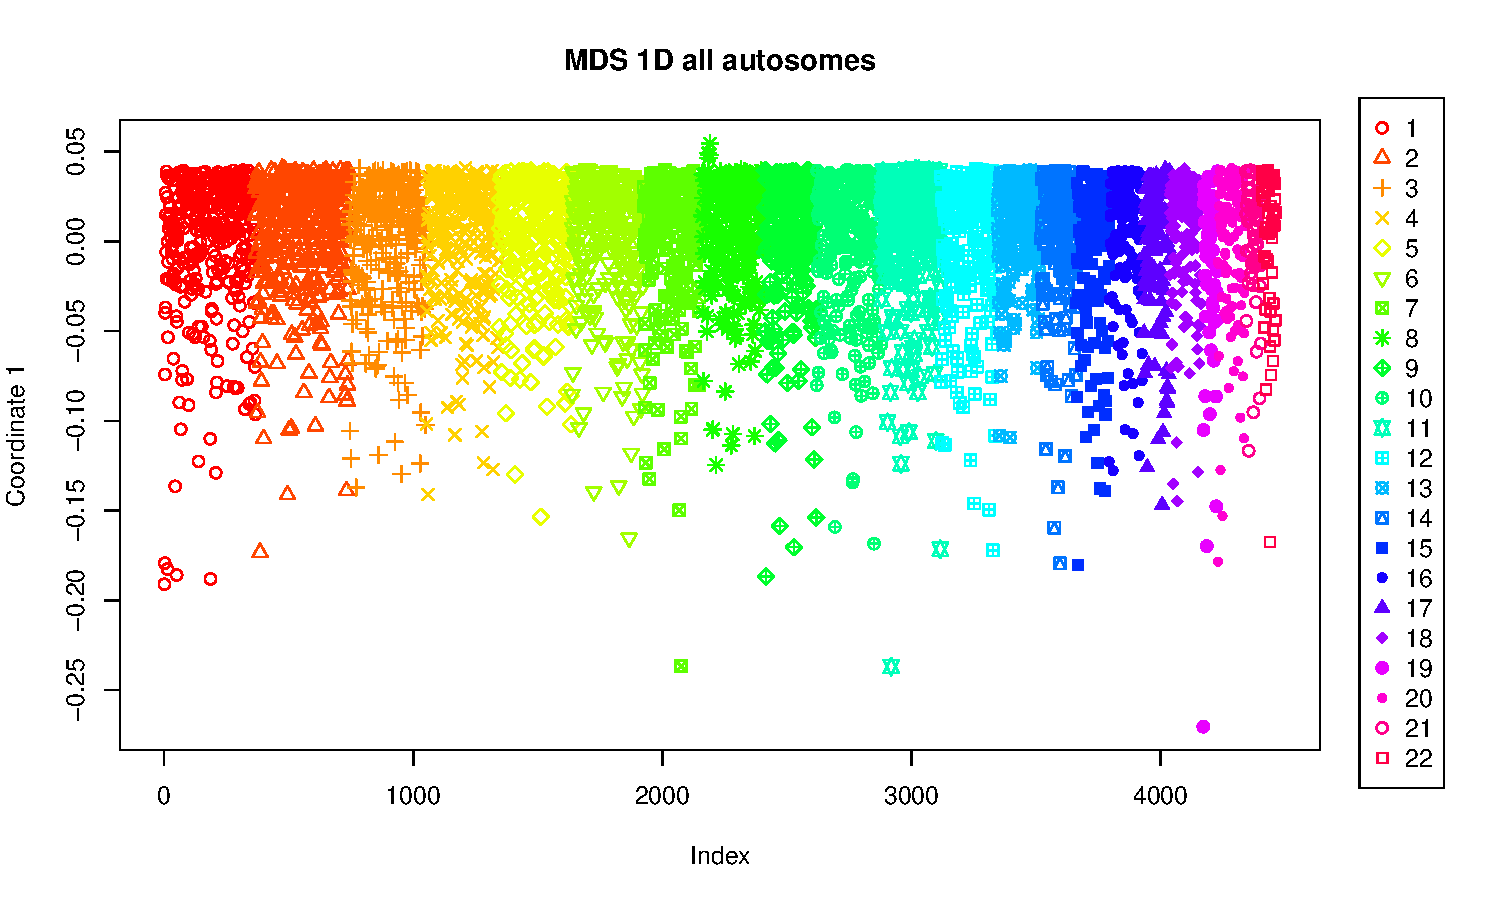
\includegraphics[width=1\textwidth]{MDS_1D_win100_all_chr_col_by_chr_with_legend}
    \end{center}
    \caption{
        MDS 1D plot along all 22 autosomes in Human.
        \label{fig:mds1_along_allchr_human}
    }
\end{figure}



\begin{figure}
    \begin{center}
       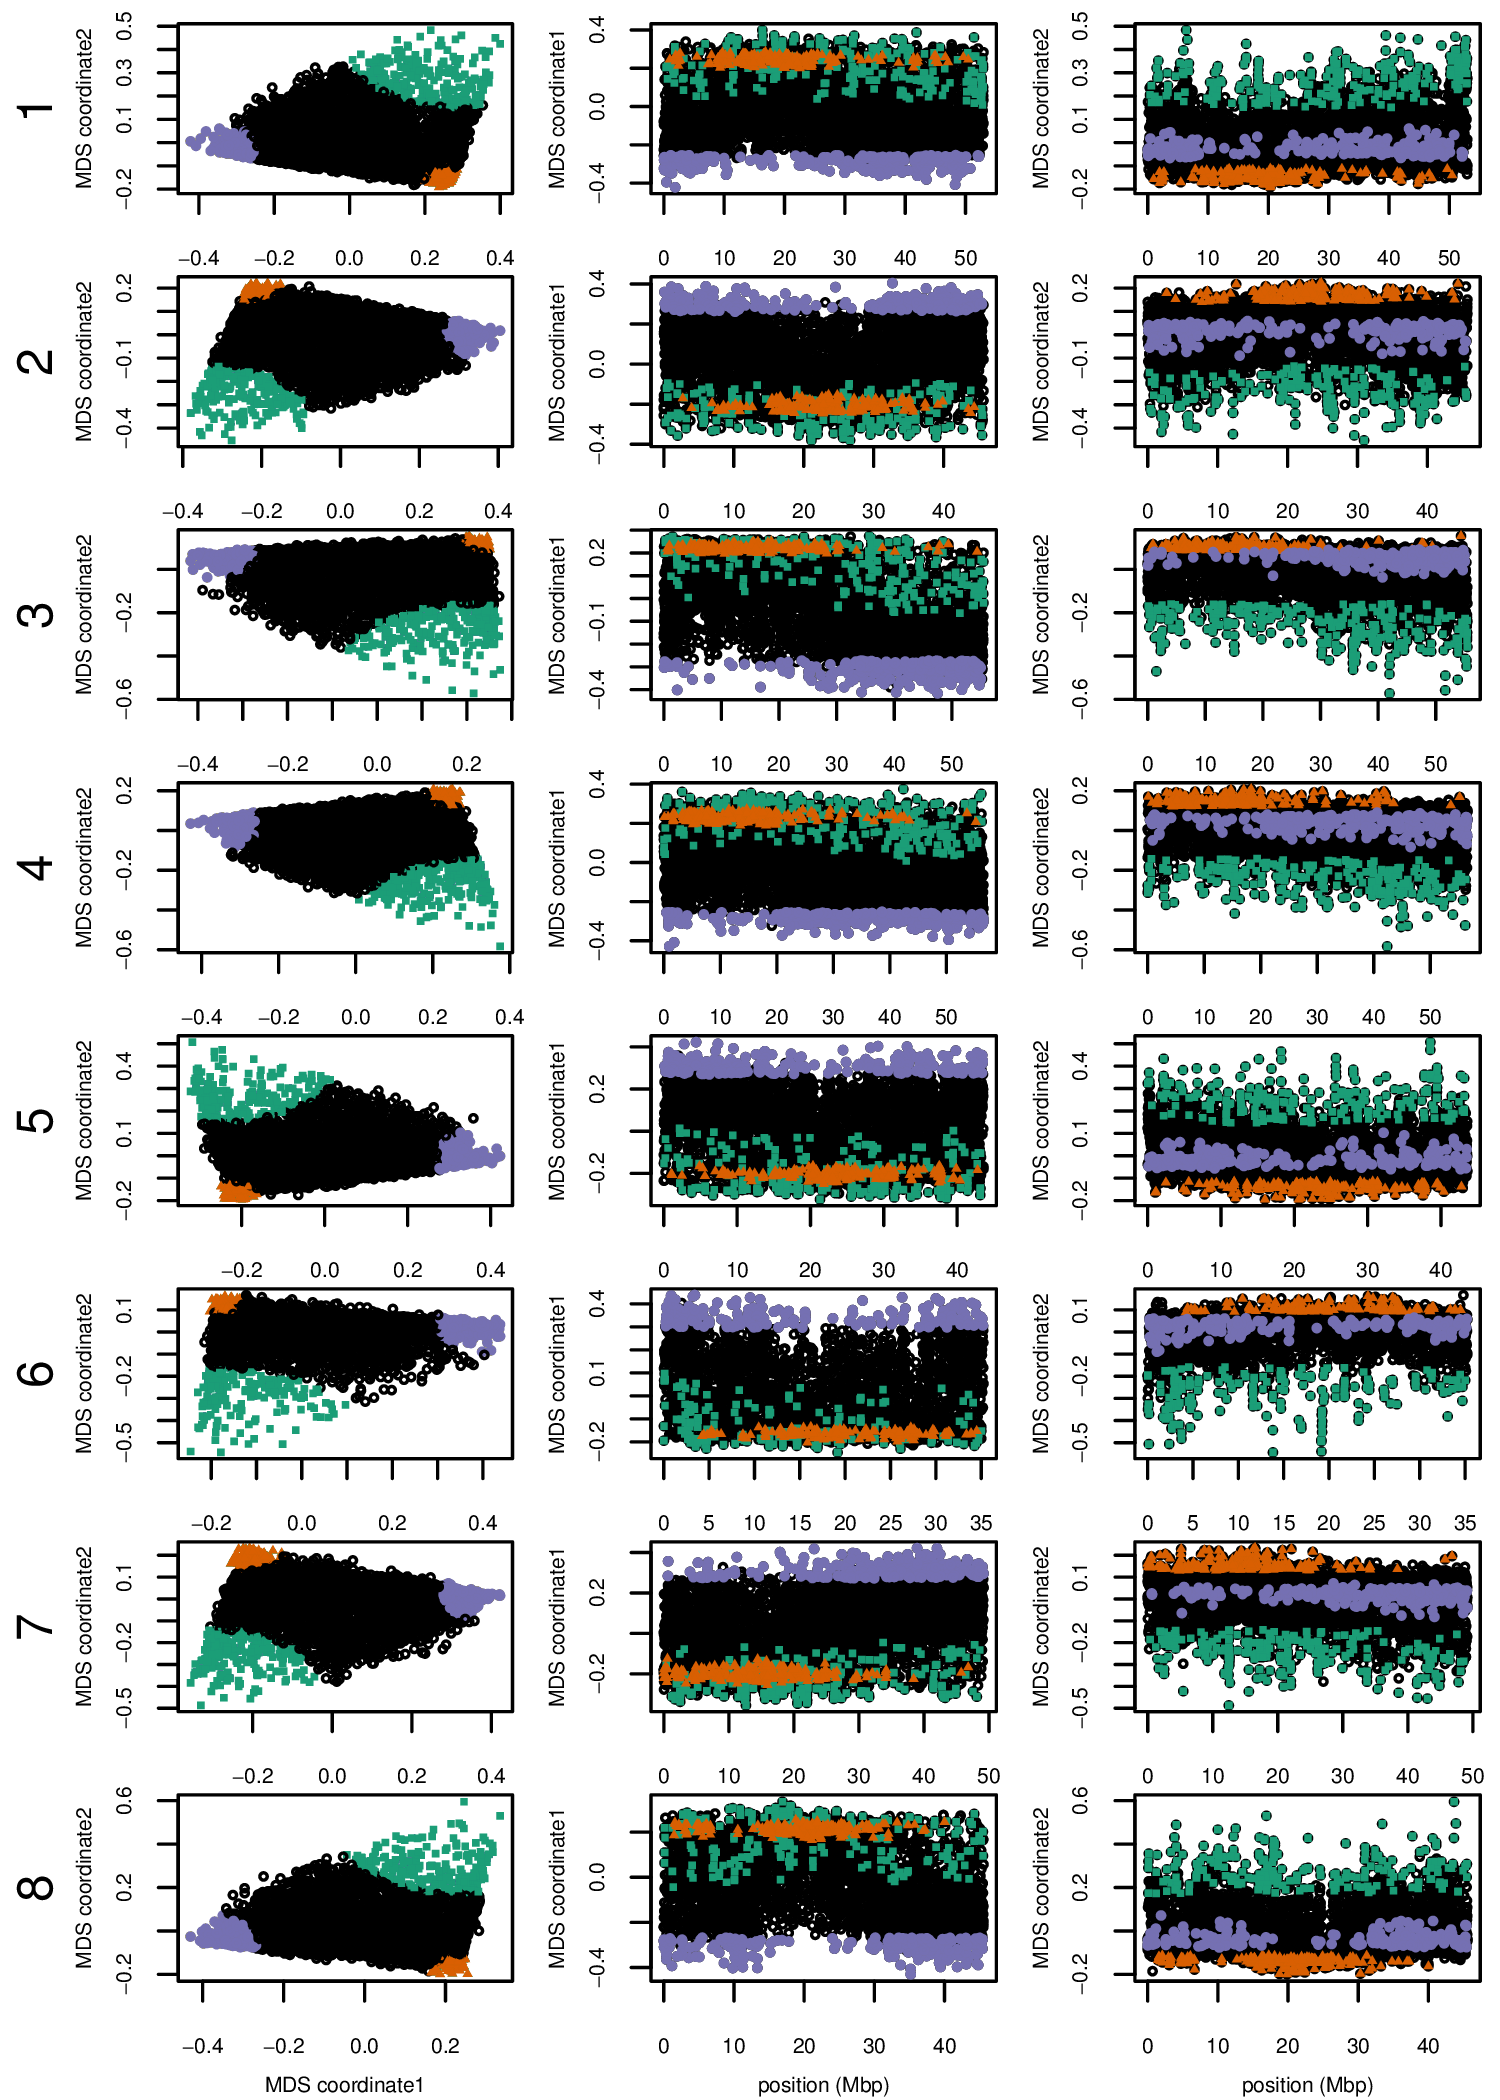
\includegraphics[width=0.85\textwidth]{FigS_Together_MDS_plot_allchr}
    \end{center}
    \caption{
        MDS plots for all 8 chromosomes in \textit{Medicago truncatula}.
        \label{fig:mds_medicago_allchr}
    }
\end{figure}


\begin{figure}
    \begin{center}
       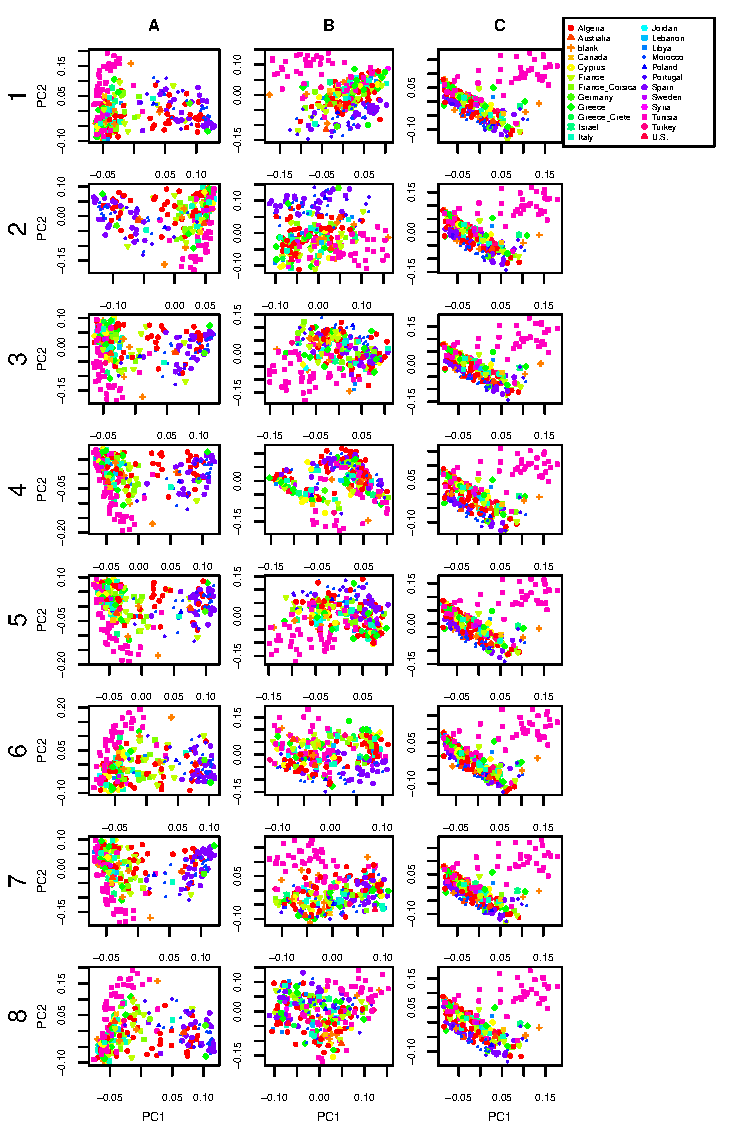
\includegraphics[width=0.82\textwidth]{FigS_pca_plots_for_Medicago_allchr_3peaks_byMDS}
    \end{center}
    \caption{
        PCA plots for all 8 chromosomes' 3 peaks in \textit{Medicago truncatula}.
        \label{fig:pca_peaks_medicago_allchr}
    }
\end{figure}

\begin{figure}
    \begin{center}
       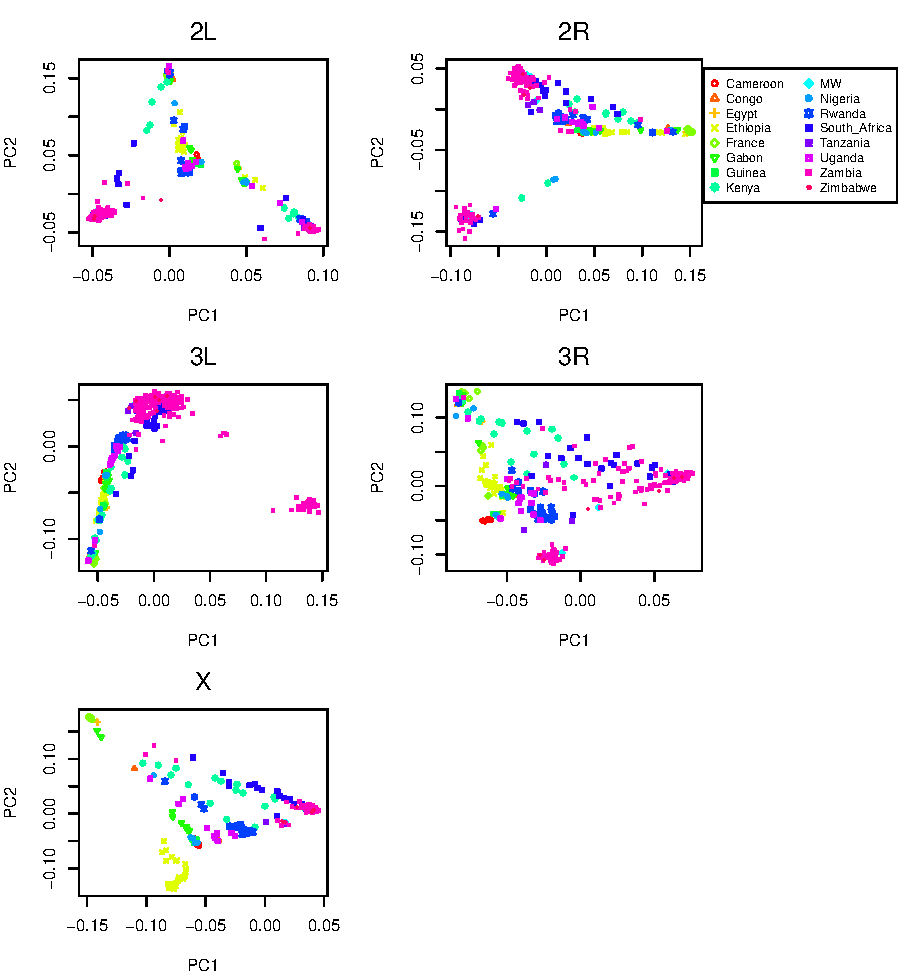
\includegraphics[width=1\textwidth]{FigS_pca_plots_allchr_drosophila}
    \end{center}
    \caption{
        PCA plots for chromosome arms 2L, 2R, 3L, 3R and X in \textit{Drosophila}.
        \label{fig:pca_drosophila_allchr}
    }
\end{figure}

\begin{figure}
    \begin{center}
       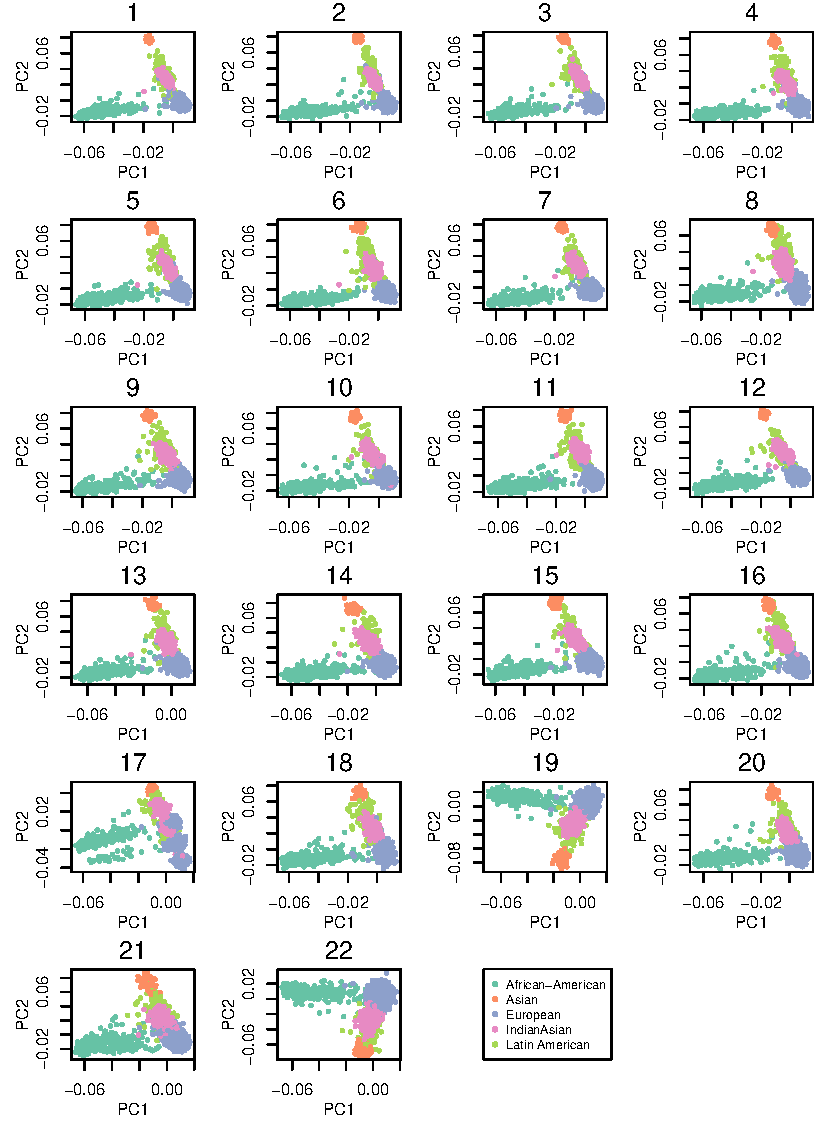
\includegraphics[width=0.9\textwidth]{FigS_pca_plot_allchr_human}
    \end{center}
    \caption{
        PCA plots for all 22 autosomes in human.
        \label{fig:pca_human_allchr}
    }
\end{figure}

\begin{figure}
    \begin{center}
       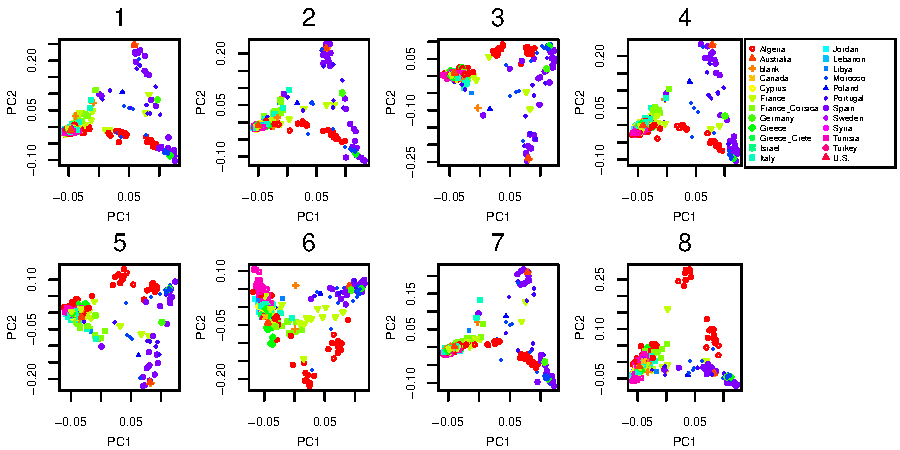
\includegraphics[width=1\textwidth]{FigS_pca_plots_medicago_allchr}
    \end{center}
    \caption{
        PCA plots for all 8 chromosomes in \textit{Medicago truncatula}.
        \label{fig:pca_medicago_allchr}
    }
\end{figure}









\end{document}  
